\chapter{Background}
\label{Background}

This chapter gives an outline of the concepts and a detailed explanation of the various technologies that will be used later in this thesis.

	\section{Containers}
	\label{Background:Containers}
	The concept of container technology uses the same model as shipping containers in transportation. The idea is that before the invention of shipping containers, manufacturers had to ship goods in a variety of fashions which included ships, trains, airplanes, or trucks, all with different sized containers and packaging.
	With the standardization of shipping containers, products could be transported seamlessly without further preparation using different shipping methods. Before the arrival of this standard, shipping anything in volume was a complex, laborious process. The motivation behind software containers is the same. \cite[P.~1]{Kinnary2018}\\

	Instead of shipping a complete operating system (OS) and the software (with necessary dependencies), we pack our code and dependencies into an image that can run anywhere. Furthermore,  it enables the packaging of clusters of containers onto a single computer. In other words, a container consists of an entire runtime environment: an application, plus all the dependencies, libraries, and other binaries, and configuration files needed to run it, bundled into one package.
	The ability to have software code packaged in pre-built software containers means that code can be pushed to run on servers running different Linux kernels or be connected to run a distributed app in the cloud. This approach also has the advantage of speeding up the testing process and creating large, scalable cloud applications. This approach has been in software development communities for several years. It has recently gained in popularity with the growth of Linux and cloud computing. \cite[P.~2]{Kinnary2018}\\
	
	% \newpage
	\subsection{Containerization vs Virtualization}
	Linux containers and virtual machines (VMs) are both package-based computing environments that combine several IT system components and keep them isolated from the rest of the system. Their main distinguishing features are scalability and portability. Containers are usually measured in megabytes, whereas VMs in gigabytes.
	\cite{containersRedHat}
	\begin{figure}[H]
		\centering
		% \input{"Bilder/tikz/Grundlagen/docker-types-of-mounts.tex"}
		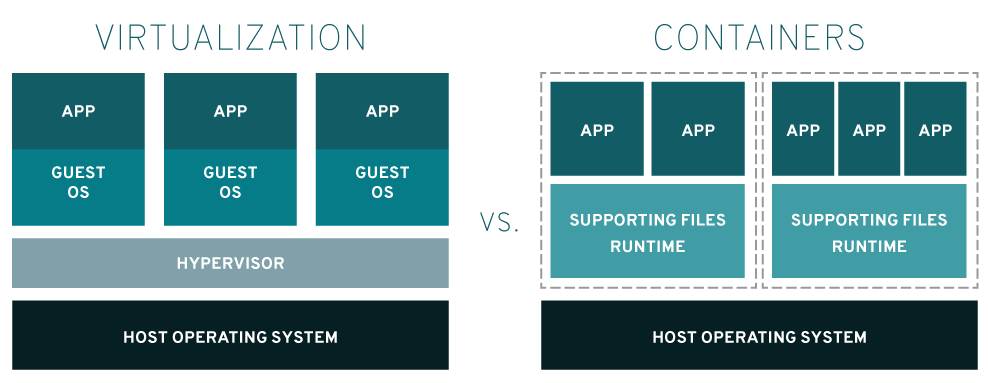
\includegraphics[width=0.9\textwidth]{"Bilder/virtualization-vs-containers_transparent.png"}
		\caption{Differences between Virtualization and Containerization \cite{containersRedHat}}
		\label{fig:Background:Containers:Containers vs VMs}					
	\end{figure}

	\paragraph*{Containerization} is an alternative to standard virtualization that encapsulates an application in a container with its executing environment.
	Containers hold an application and everything it needs to run. Everything within a container is maintained on an image—a code-based file that includes all libraries and dependencies. These files are similar to a Linux distribution installation. An image comes with RPM packages and configuration files. Containers are so small compared to VMs, there are usually hundreds of them loosely coupled together.\cite{containersRedHat}
	
	\paragraph*{Virtualization} is a way of sharing a single physical instance of a resource or an application to multiple organizations and clients. It utilizes software called a hypervisor that separates resources from their physical devices. It enables the partitioning of the resources and assigned to individual VMs. When a user issues a VM instruction that requires additional resources from the physical environment, the hypervisor sends the request to the physical system and saves the changes. VMs look and act like physical servers, which can multiply the drawbacks of application dependencies and large OS footprints—a footprint that's often not required to run a single app or microservice.\cite{containersRedHat} \\

	Table \ref{tab:container_vs_vms} illustrates the key differences between the above two approaches concerning package-based computing environments.
	\begin{table}[H]
        \centering
		\rowcolors{1}{}{gray!25}
        \begin{tabular}{{p{3cm}|p{5cm}|p{6cm}}}
            \toprule
            Parameters & Virtualization & Containerization\\
            \midrule
            Isolation & Provides complete isolation from the host operating system and the other VMs & Provides lightweight isolation from the host and other containers, but doesn’t provide a strict security boundary as a VM \\
            Operating System & Runs a complete operating system including the kernel, thus requiring more system resources such as CPU, memory, and storage & Runs the user-mode portion of an operating system, and can be customized to include just the required services for your app utilizing fewer system resources \\
            Compatibility & Runs just about any operating system inside the virtual machine & Runs on the same operating system version as the host\\
            Deployment  & Deploys individual VMs by using Hypervisor & Deploys single container by using Docker or deploy multiple containers by using an orchestrator such as Kubernetes\\
            Persistent storage  & Uses a Virtual Hard Disk (VHD) for local storage for a single VM or a Server Message Block (SMB) file share for storage shared by multiple servers & Uses local disks for local storage for a single node or SMB for storage shared by multiple nodes or servers\\
            Networking  & Uses virtual network adapters & Uses an isolated view of a virtual network adapter. Thus, providing a little less virtualization\\
            Startup time & They take few minutes to boot up & They can boot up in few seconds \\
            \bottomrule
        \end{tabular}
		\caption{Differences between Virtualization and Containerization \cite{containers-vs-vms-Baeldung}}
		\label{tab:container_vs_vms}
    \end{table}

		\paragraph{Image}
			Ein Docker-Image ist ein Speicherabbild eines Containers. 
			Das Image besteht aus mehreren Layern, die schreibgeschützt sind.
			Images können manuell erstellt werden, oder mit Verwendung eines dockerfiles automatisiert kompilliert werden.
			
		\paragraph{Container}
			Ein Container ist die aktive ausgeführte Instanz eines Images.
			Es läuft immer ein Prozess innerhalb des Containers.
			Somit wird ein Container beendet, sobald er kein Programm ausführt oder das Programm mit seinem Auftrag fertig ist.
			
		\paragraph{Dockerfile}
			Ein Dockerfile ist eine Textdatei mit Anweisungen zum erstellen eines Containers.
			Jeder Schritt erstellt einen neuen Layer, der dem Image hinzugefügt wird.
			Mit einem Dockerfile lässt sich das erstellen von Images automatisieren.
		
		\paragraph{Docker-Compose}
			Mit Docker-Compose lassen sich die Startparameter eines Containers in einer .yaml -Datei festlegen.
			Es lassen sich mehrere Docker-Container gleichzeitig starten, sowie umfangreiche Einstellungen bei dem Start des Containers treffen.
		
		\subsection{Netzwerke}
		\label{Grundlagen:Docker:Netzwerke}
			Docker bietet auch die Netzwerkkapselung für die Container an.
			Somit lässt sich das Netzwerk eines Containers von dem Rest des Systems oder anderen Containern trennen.
			Es können auch eigene Netzwerke definiert werden, um mehrere Container miteinander Kommunizieren zu lassen.
			Sie spannen so ein eigenes Netzwerk auf, was vergleichbar mit einem lokalen Netzwerk ist.
			Zwei Netzwerktypen die Docker anbietet, werden nachfolgend erläutert.
			\paragraph{Bridged}
				Das Bridged Netzwerk kapselt das Netzwerk des Containers von dem des Host Systems, bietet aber noch eine Netzwerk-Brücke, damit der Container Teilnehmer in höherliegenden Netzen erreichen kann.
				Es lassen sich Ports des Host-Computers an einen Container weiterleiten, um so eine Erreichbarkeit des Containers aus einem höherliegendem Netz zu ermöglichen.
				
			\paragraph{Host}
				Die Netzwerkeinstellung Host verzichtet auf eine Kapselung der Netze.
				Hier verwendet der Container die IP Adresse des Host-Computers und ist entsprechend teil des Host-Netzes.
				Für weitere Teilnehmer des Netzwerkes, ist der Host-PC des Docker-Containers und der Container selbst, dasselbe Gerät.
				Eine Portweiterleitung zum ermöglichen von Diensten ist hier nicht notwendig.
				
			\subsection{Datenspeicherung}
			\label{Grundlagen:Docker:Datenspeicherung}
				Nach beenden des Containers werden die Daten, die während dem ausführen des Containers angefallen sind, gelöscht.
				Um eine Persistente Speicherung, zu ermöglichen, bietet Docker mehrere Möglichkeiten an, um über die Laufzeit des Containers hinaus Daten zu speichern, oder auch um auf Daten innerhalb des Containers zuzugreifen. 
				Nachfolgend werden die wichtigsten kurz vorgestellt.
				
				\begin{figure}[H]
					\centering
					% \input{"Bilder/tikz/Grundlagen/docker-types-of-mounts.tex"}
					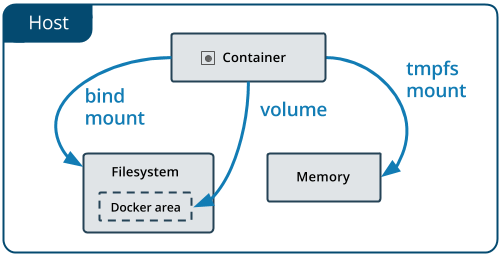
\includegraphics[width=0.70\textwidth]{"Bilder/DockerSpeichertypenpng.png"}
					\caption{Verschiedene Datenspeichermöglichkeiten. \cite{dockerStorage}}
					\label{fig:Grundlagen:Docker:Datenspeicherung}					
				\end{figure}
										
				\paragraph{Volumes}
					Volumes werden auf dem Dateisystem des Hosts gespeichert (In Linux unter \textit{/var/lib/docker/volumes/}).
					Ein Volume kann in mehrere Container eingebunden werden, dadurch ist eine containerübergreifende Dateiablage möglich.
					Volumes werden nicht automatisch gelöscht, sobald alle Container gestoppt sind, welches das Volume eingebunden hatten.
					Sie eignen sich am besten, um Daten Persistent zu speichern. \cite{dockerStorage}
				
				\paragraph{Bind mounts}
					Bind mounts können überall auf dem Hostsystem gespeichert sein.
					So können wichtige Systempfade (zum Beispiel \textit{/dev/}) dem Container zugänglich gemacht werden. \cite{dockerStorage}
				
				\paragraph{tmpfs mounts}
					Hier werden die Dateien nicht auf dem Dateisystem des Hosts gespeichert, sondern auf dem Arbeitsspeicher des System.
					Dadurch entsteht eine nicht persistente Datenspeicherung, um geheime Informationen zwischen Containern auszutauschen. \cite{dockerStorage}
					
				
	\section{Industrial Edge}
	\label{Grundlagen:IndustrialEdge}
		Industrial Edge ist eine Entwicklung von Siemens, die ermöglicht, im Prozess anfallende Daten bereits auf dem Gerät zu analysieren.
		Es wird lokales Engineering mit Cloud Engineering kombiniert. \cite{siemensIEM_gettingStarted}
		Dadurch werden unnötige Datentransporte zwischen dem Endgerät und Server vermieden und erst bereits aufbereitete Daten zum Server geschickt.
		Die Rechenlast fließt so vom Server in Richtung des Endgerätes.
		Hierfür werden Applikationen (Apps) bereitgestellt, die einen festen Funktionsumfang enthalten und mit der Industrial Edge Infrastruktur auf das jeweilige Endgerät (Edge Device) gespielt werden können.
		Diese Apps basieren auf der Docker Technologie.
		Industiral Edge ermöglicht die zentrale Verwaltung von
		In der nachfolgenden Abbildung \ref{fig:Grundlagen:IndustrialEdge:Ueberblick} ist eine typische Infrastruktur von dem obersten Server, bis zu den Endgeräten dargestellt, die im Nachfolgenden näher erläutert wird.
		\begin{figure}[h]
			\centering
			%\input{"Bilder/tikz/Grundlagen/industrial-edge-overwiev.tex"}
			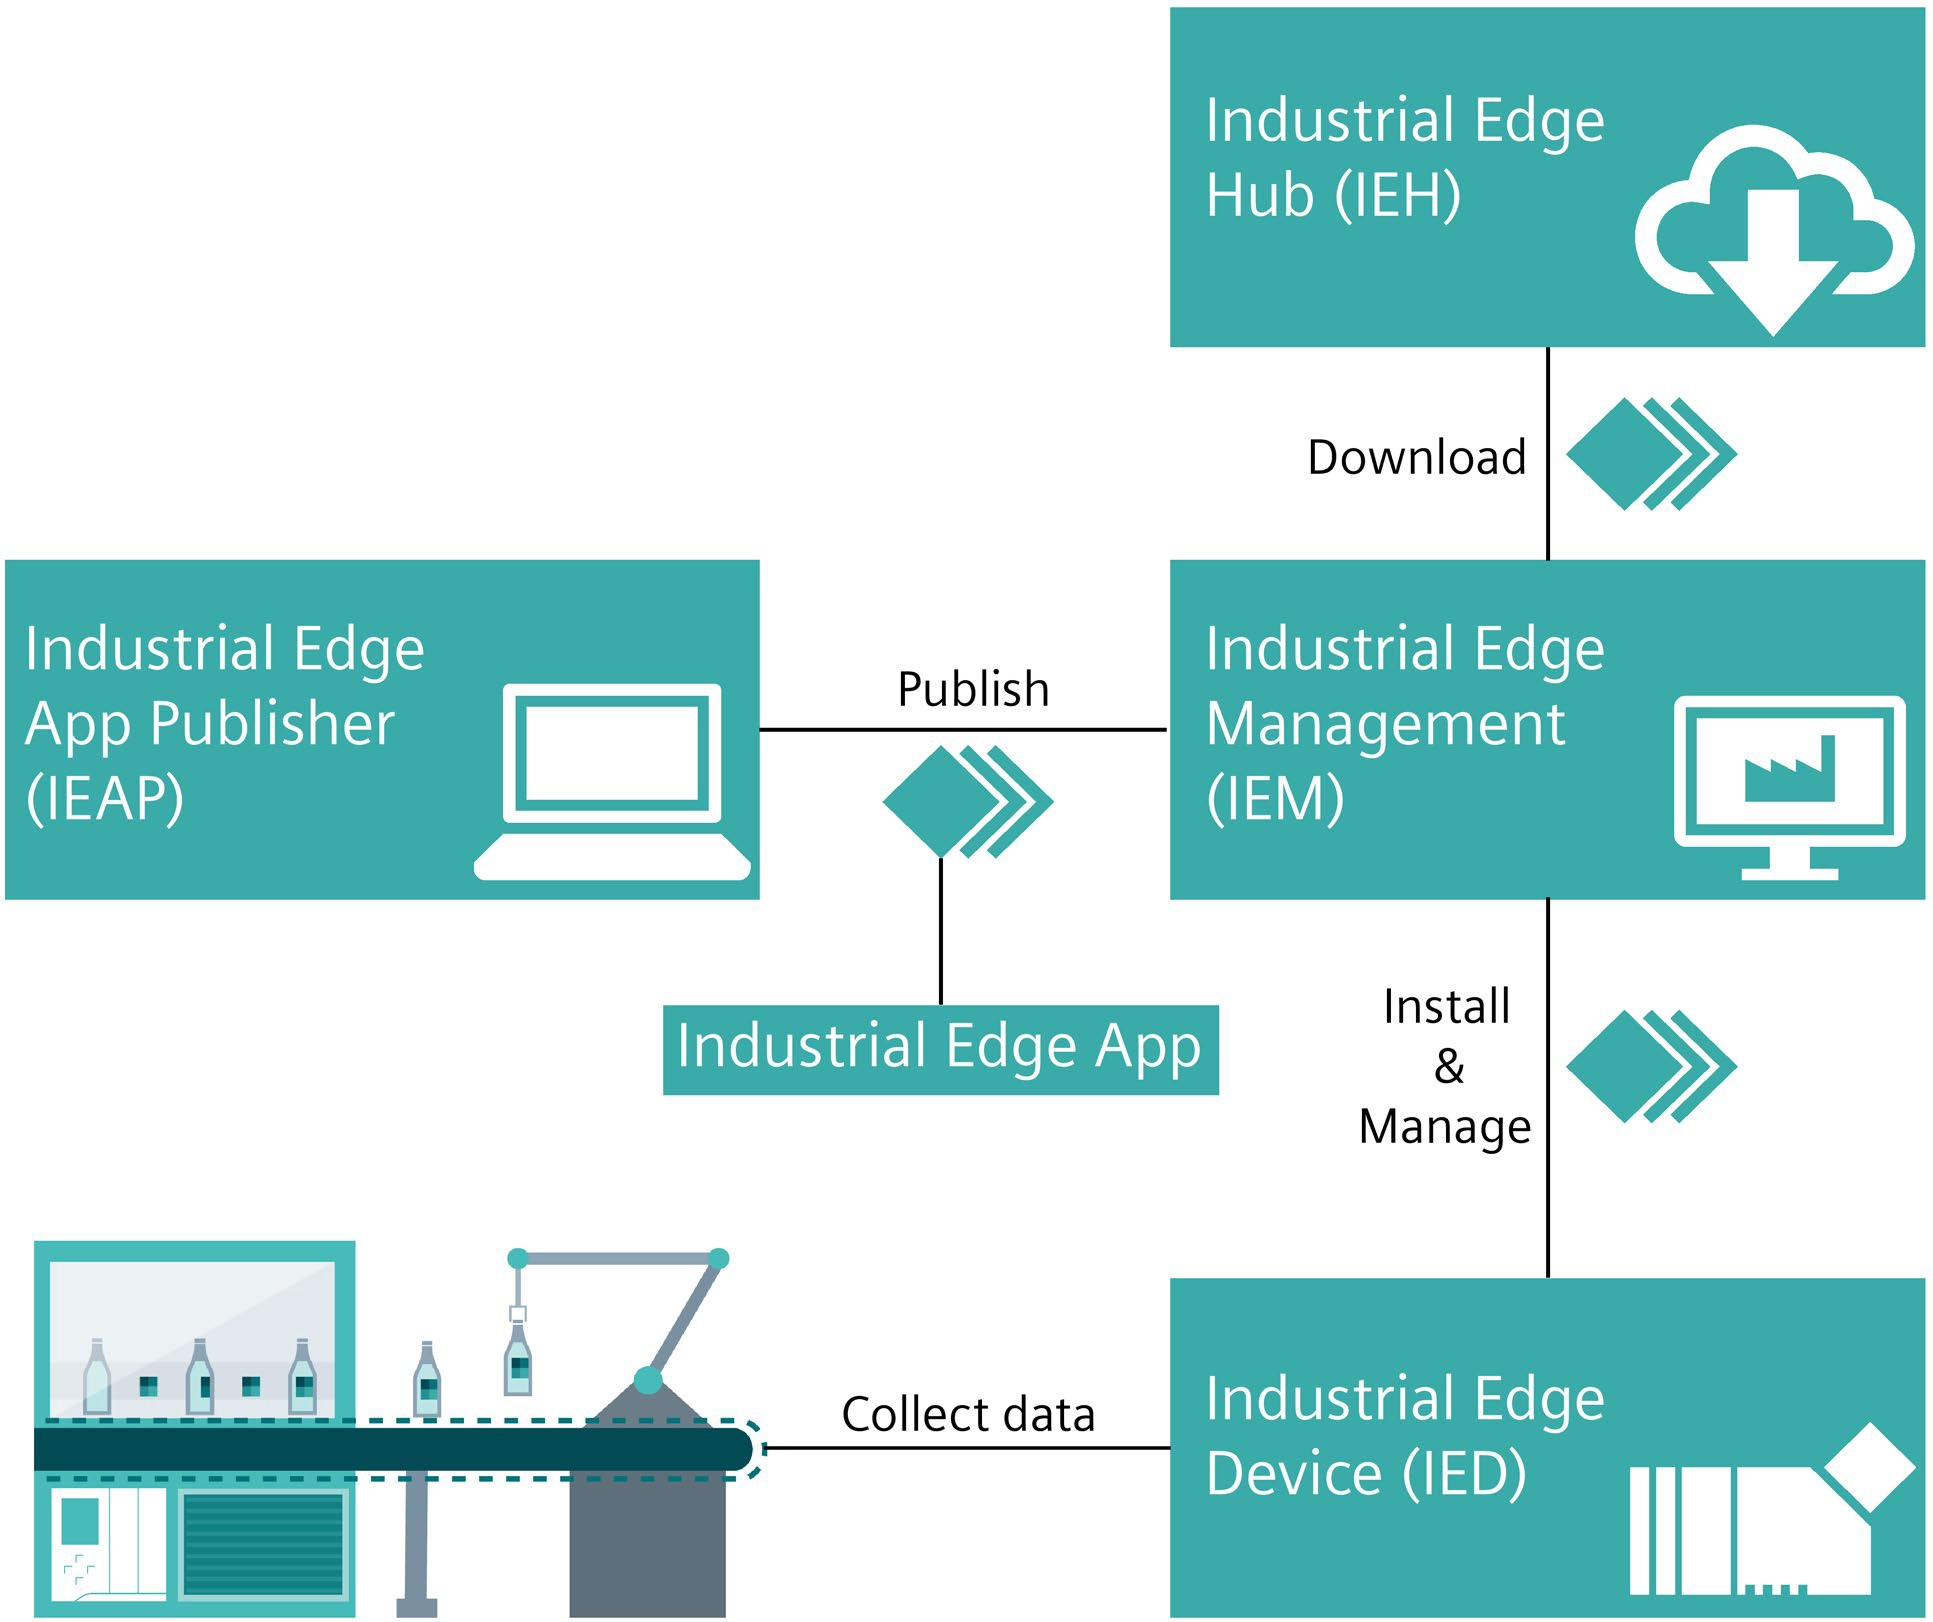
\includegraphics[width=0.70\textwidth]{"Bilder/Edge_uebersicht.jpg"}
			\caption{Überblick über Industrial Edge. \cite{siemensIEM_gettingStarted}}
			\label{fig:Grundlagen:IndustrialEdge:Ueberblick}					
		\end{figure}
	
		%- Management tool für Docker Container auf Geräten (Device)\\
		%- Graphen die das IE-Hub, IEM, Docker Device erklärt\\
			
		\paragraph{Industrial Edge Hub}
			Das \gls{IEH} ist die oberste, von Siemens bereitgestellte Serverebene.
			Hier bietet Siemens eigene entwickelte Applikationen an, die gegen eine Lizenzgebühr auf das \gls{IEM} geladen werden können.
			Von hier aus lassen sich ebenfalls benötigte Softwarepakete und Dokumentation herunterladen, die das Entwickeln von eigenen Apps und das Aufsetzen und betreiben von einem eigenen \gls{IEM} ermöglicht. \cite{siemensIEM_gettingStarted}
			
		\paragraph{Industrial Edge Management System}
			Das \gls{IEM} ist ein Server, welcher in einem Lokalen Netz selbstständig betrieben werden kann.
			Der Anwender hat hiermit die Möglichkeit, einen Server zu erstellen, damit z.B. sensible Daten, die zwischen dem Edge Device und dem \gls{IEM} ausgetauscht werden, nicht über das Internet transportiert werden müssen.
			Zudem lassen sich die Endgeräte über diesen Server verwalten, es können Apps sowie Softwareupdates aufgespielt werden, sowie lassen sich weitere Analysen durchführen.
			Eine selbst entwickelte App lässt sich auf das \gls{IEM} aufspielen, welches Diese wiederum an die Edge Devices verteilen kann.
			\cite{siemensIEM_gettingStarted}
			
		\paragraph{Industrial Edge App}
			Eine Edge App dient zur intelligenten Verarbeitung von Automatisierungsaufgaben. \cite{siemensIEM_gettingStarted}
			Neben den von Siemens im \gls{IEH} angebotenen Apps lassen sich auch eigene Applikationen entwickeln.
			Diese und eigene entwickelte Apps sind Docker basierte Images, welche auf dem \gls{IED} ausgeführt werden.
			Als oberste Beschreibungsebene wird eine docker-compose Datei angelegt, in welcher beschrieben wird, wie die docker Images zu starten sind, sowie welche Netzwerkkonfiguartion (Kapitel \ref{Grundlagen:Docker:Netzwerke}) und welche Art der Datenspeicherung (Kapitel \ref{Grundlagen:Docker:Datenspeicherung}) verwendet wird.
	
		\paragraph{Edge Device}
			Ein \gls{IED} führt die einzelnen Edge Apps aus. Sie können Automatisierungsdaten lokal speichern und nach Bedarf abrufen. 
			Ebenfalls lassen sich diese Daten an eine Cloud-Infrastruktur übermitteln. Ein \gls{IED} muss bei einem \gls{IEM} aktiviert werden.
			\cite{siemensIEM_gettingStarted}
			
		\paragraph{Industrial Edge Publisher}
			Der Industrial Edge Publishers ist ein Tool, mit dem Docker Images in Edge Apps überführt und in das \gls{IEM} hochgeladen werden.
			Es lassen sich ebenfalls bereits erstellte Apps verwalten, verändern oder löschen.
			\cite{siemensIE_App}

	
	\section{ROS 2}
	\label{Grundlagen:ROS2}
		Ein asdfasdasd
		\cite{ros2Basic}
		\gls{ROS2}
	
	
	
		\subsection{Nachrichtentypen}
		\label{Grundlagen:ROS2:Nachrichtentypen}
			- Message (topics)\\
			- Service\\
			- Action
			
		\subsection{ROS 2-web Bridge}
		\label{Grundlagen:ROS2:2WebBridge}
			- Stellt einen websocket bereit, der mittels JSON requests verarbeitet. 
			- Basiert auf RclNodeJS, welches eine brücke zwischen javascript und ros2 bildet\\
			- Basiert auf NodeJS. NodeJs ist eine JavaScript Runtime, die JS Code serverseitig ausführen lässt.
			Das ist hier nicht weiter von relevanz.\\
			- Verwendet wird für die Anwendung ebenfalls roslibjs. Dies ist eine javascript bibliothek, welche in der html eingebunden wird. Sie stellt Befehle zum erstellen von ROS Subscriber/Publisher und Services bereit.\\
			
		\subsection{roslibjs}
		\label{Grundlagen:ROS2:RosLibJS}
	
	\section{DDS}
	\label{Grundlagen:DDS}
		- Grundlage für Kommunikation von ROS2\\
		- Realisiert die eigentliche Kommunikation\\
		- Wenn das hier geht, geht auch ROS2!
		- Verschiedene Systemanbieter, näher wird RTI und Fastrtps untersucht: https://ros.org/reps/rep-2000.html  (Beide TIER 1)
		
		ROS2 verwendet als Kommunikationsschnittstelle DDS.
		DDS funktioniert gut in lokalen Netzwerken, sobald allerdings ein NAT-Router dazwischen ist, funktioniert der standardmäßige Discovery Mechanismus nicht.
		Da das Ziel eine Edge Applikation ist, soll das Verhalten von DDS in der Docker Umgebung, bzw. in unterschiedlichen Netzwerken untersucht werden.
	
		
		
